\section{\texorpdfstring{Popis protokolu}{Popis protokolu}}

% =====================================================================================================================
	\begin{frame}
    \frametitle{Historie a použití}
		\small
		
		\begin{itemize}
			\item Protokol vytvořila firma MODICON v roce 1979,
			\item byl určen pro DCS (\textbf{D}istributed \textbf{C}ontrol \textbf{S}ystem), tj. více spolupracujících stanic (PLC) se podílí na řízení technologického procesu:
			
			\begin{itemize}
				\item jednotlivé části technologie mají vlastní řídicí jednotku,
				\item systémy spolu komunikují po průmyslové síti,
			\end{itemize}
			
			\item primárně byl určen pro sériovou komunikaci - Modbus RTU, 
			\item v roce 1999 přibyla podpora ethernetové komunikace - Modbus TCP,
			\item komunikace probíhá v režimu master-slave:
			
			\begin{itemize}
				\item \textbf{master} zadává dotazy nebo příkazy,
				\item \textbf{slave} odpovídá nebo provádí akce.
			\end{itemize}
		\end{itemize}
		
	\end{frame}
	
	% =====================================================================================================================
	\begin{frame}
    \frametitle{Typický DCS}
		
		\begin{center}
			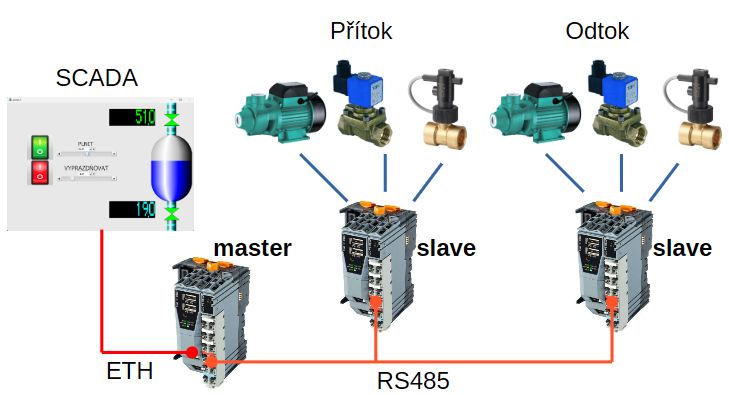
\includegraphics[width=1.00\textwidth]{fig/DCS.png}
		\end{center}
	
	\end{frame}
	
% =====================================================================================================================
	\begin{frame}
    \frametitle{Datový model}
		
		\begin{itemize}
			\item Protokol je založen na poskytování dat ve formě tabulek (nebo lépe paměťového prostoru),
			\item typický má paměťový prostor 4 oblasti (bloky paměti):
		\end{itemize}
		
		\begin{center}
			\small
			\begin{tabular}{| c | c | p{50mm} |}
			\hline
				\textbf{Adresa} & \textbf{Typ hodnoty} & \textbf{Vztah k PLC} \\ \hline
				00001 - 09999 & Cívky & odpovídají digitální výstupy \\ \hline
				10000 - 19999 & Diskrétní vstupy & digitální vstupy \\ \hline
				30000 - 39999 & Vstupní registry & analogové vstupy \\ \hline
				40000 - 49999 & Uchovávací registry & analogové výstupy \\ \hline
			\hline
			\end{tabular}
		\end{center}
		
		\begin{itemize}
			\item analogové hodnoty mají vždy rozlišení 16 bitů,
			\item diskrétní hodnoty jsou jednobitové.
			\item \textcolor{red}{\textbf{POZOR:}} je rozdíl mezi fyzickou a logickou adresací:
			
			\begin{itemize}
				\item při \textbf{logické adresaci} má první buňka adresu \textbf{1}, zatímco
				\item při \textbf{fyzické adresaci} má první buňka adresu \textbf{0}.
			\end{itemize}
		\end{itemize}
	\end{frame}
	
% =====================================================================================================================
	\begin{frame}
    \frametitle{Formát zprávy}
		
		\begin{center}
			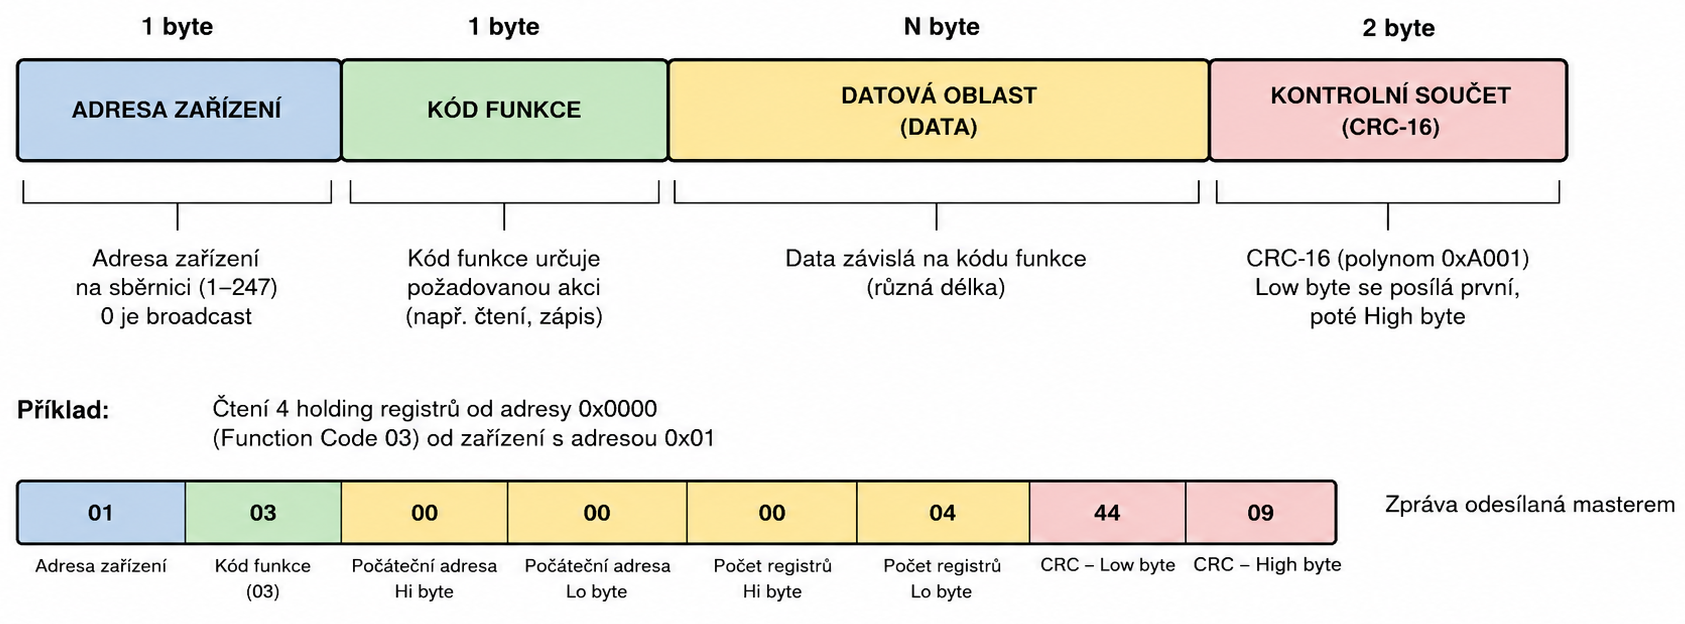
\includegraphics[width=1.00\textwidth]{fig/format_zpravy.png}
		\end{center}
		
		\small
		
		\begin{itemize}
			\item Data mají reprezentaci Big Endian,
			\item CRC má reprezentaci Little Endian,
		\end{itemize}
		
	\end{frame}
  
% =====================================================================================================================
	\begin{frame}
    \frametitle{Oddělení jednotlivých zpráv}
		
		\begin{center}
			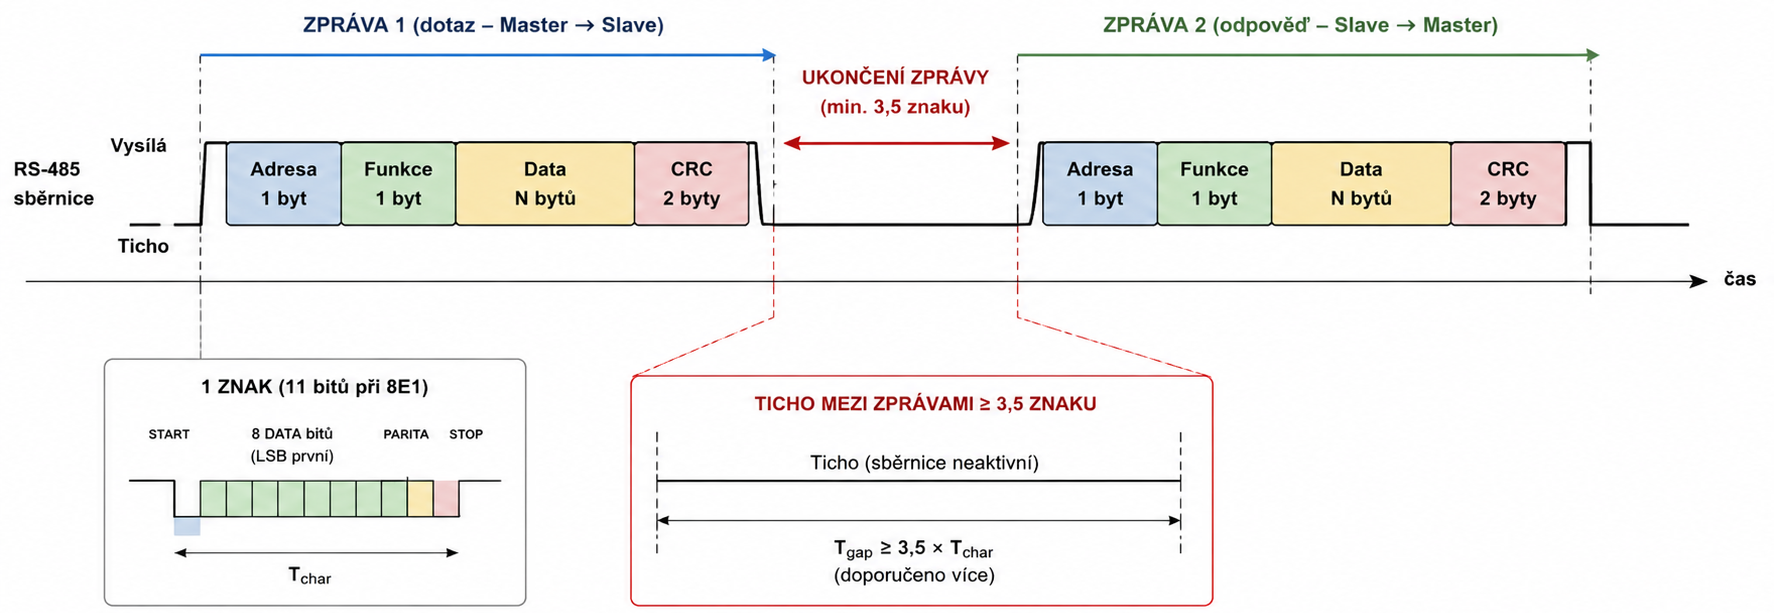
\includegraphics[width=1.00\textwidth]{fig/deleni_zprav.png}
		\end{center}
		
		\small
		
		\begin{itemize}
			\item Klid na lince 3.5 znaku odděluje jednotlivé zprávy nebo ruší předchozí vysílání,
		\end{itemize}
		
		\textbf{POZNÁMKA:} Pro Modbus RTU je velmi typické nastavení sériové linky se sudou paritou.
		
	\end{frame}

% =====================================================================================================================
	\begin{frame}
    \frametitle{Nejběžnější kódy funkcí}
		\small
		\begin{center}
			\begin{tabular}{|c|p{10cm}|}
			\hline
			\textbf{Kód} & \textbf{Význam} \\ \hline

			\textcolor{blue}{01} & \textcolor{blue}{Read Coils – čtení stavů binárních výstupů (coil)} \\ \hline

			\textcolor{blue}{02} & \textcolor{blue}{Read Discrete Inputs – čtení binárních vstupů pouze pro čtení} \\ \hline

			\textcolor{blue}{03} & \textcolor{blue}{Read Holding Registers – čtení holding registrů} \\ \hline

			\textcolor{blue}{04} & \textcolor{blue}{Read Input Registers – čtení vstupních registrů pouze pro čtení} \\ \hline

			\textcolor{blue}{05} & \textcolor{blue}{Write Single Coil – zápis jednoho binárního výstupu} \\ \hline

			\textcolor{blue}{06} & \textcolor{blue}{Write Single Register – zápis jednoho holding registru} \\ \hline

			08 & Diagnostics – diagnostické funkce sériové linky \\ \hline

			\textcolor{blue}{15} & \textcolor{blue}{Write Multiple Coils – zápis více binárních výstupů} \\ \hline

			\textcolor{blue}{16} & \textcolor{blue}{Write Multiple Registers – zápis více holding registrů} \\ \hline

			22 & Mask Write Register – maskovaný zápis do registru \\ \hline

			23 & Read/Write Multiple Registers – současné čtení a zápis více registrů \\ \hline

			43/14 & Encapsulated Interface Transport – identifikace zařízení (Read Device Identification) \\ \hline

			\end{tabular}
		\end{center}
		
	\end{frame}
	
% =====================================================================================================================
	\begin{frame}
    \frametitle{Adresa zařízení a CRC}
		
		\textbf{Adresa zařízení:}
		
		\begin{itemize}
			\item Číslo v rozmezí 1-247 (0 je broadcast, 248 až 255 jsou rezervované),
			\item musí být unikátní pro konkrétní stanici.
		\end{itemize}
		
		\vspace{3mm}
		
		\textbf{Cyclic Redundancy Check:}
		
		\begin{itemize}
			\item metoda pro detekci chyb přennosu dat,
			\item modbus používá CRC-16,
			\item počítá se ze všech bytů zprávy při vysílání i příjmu,
			\item přijímač porovnává CRC ve zprávě s tím, které bylo vypočteno.
		\end{itemize}
		
	\end{frame}
	
% =====================================================================================================================
	\begin{frame}
    \frametitle{Příklad posílání jednotlivých bitů}
		
		\begin{center}
			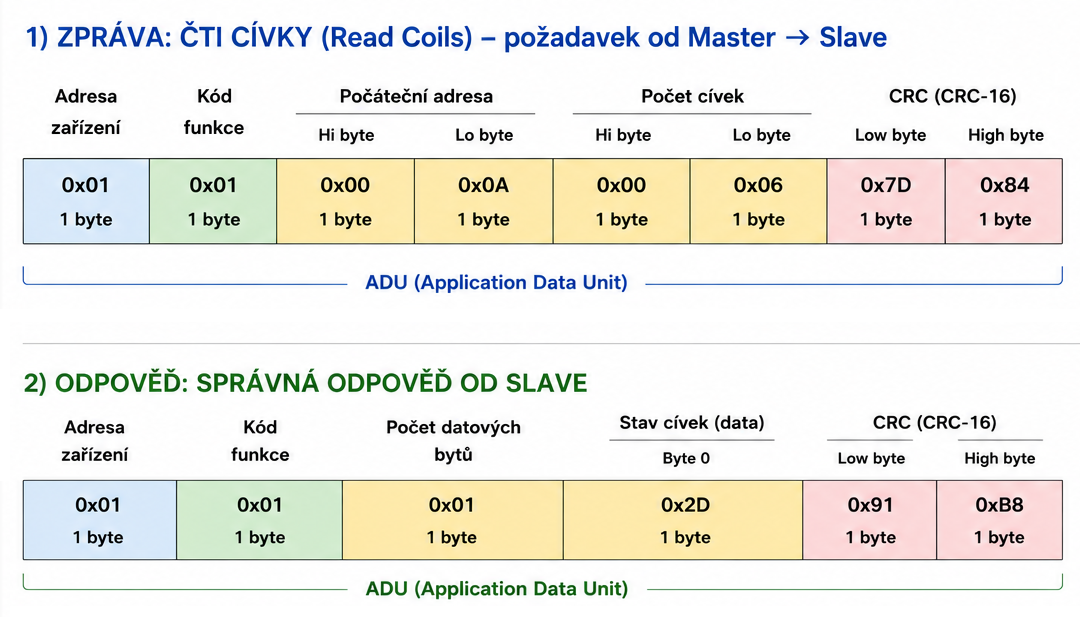
\includegraphics[width=0.80\textwidth]{fig/odpoved_OK.png}
		\end{center}
		
		\small
		\begin{itemize}
			\item Čtení 6 cívek od adresy 10,
			\item cívky mají stav $(101101)_2$ v pořadí \textbf{LSB$\rightarrow$MSB}.
		\end{itemize}
	\end{frame}
	
% =====================================================================================================================
	\begin{frame}
    \frametitle{Příklad výjmky}
		
		\begin{center}
			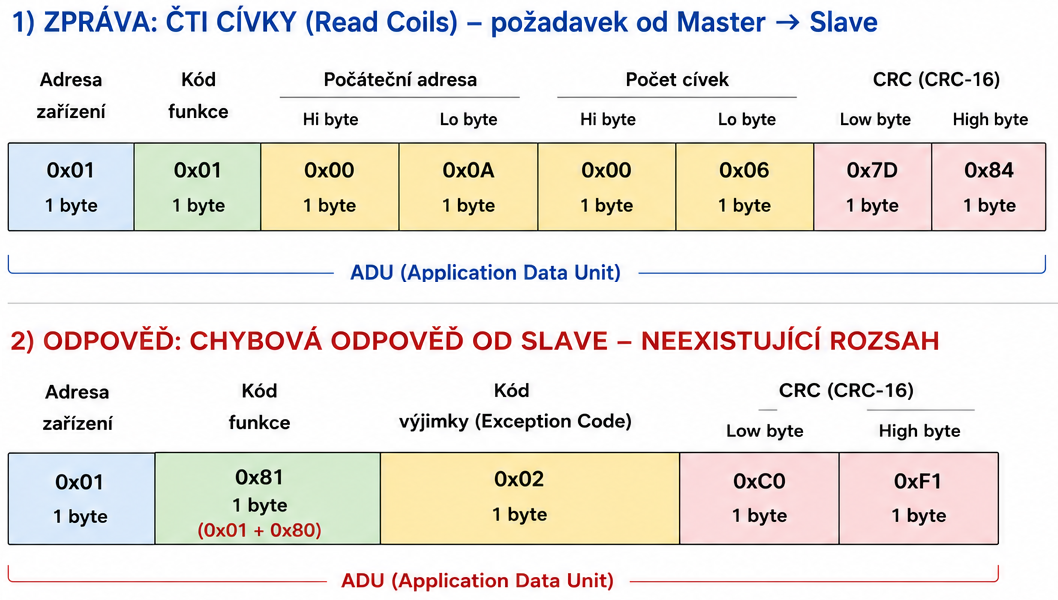
\includegraphics[width=0.80\textwidth]{fig/odpoved_ERR.png}
		\end{center}
		
		\small
		\begin{itemize}
			\item Kód funkce = požadovaný kód + 0x80,
			\item v datech je předán kód výjimky.
		\end{itemize}
	\end{frame}
	
% =====================================================================================================================
	\begin{frame}
    \frametitle{Běžné kódy výjimek}
		
		\small
		\begin{tabular}{|c|p{10cm}|}
			\hline
			\textbf{Kód} & \textbf{Význam} \\ \hline

			01 & Illegal Function -- zařízení nepodporuje požadovaný funkční kód \\ \hline

			02 & Illegal Data Address -- požadovaná adresa nebo rozsah registrů/cívek neexistuje \\ \hline

			03 & Illegal Data Value -- neplatná hodnota parametru v požadavku \\ \hline

			04 & Slave Device Failure -- interní chyba zařízení při zpracování požadavku \\ \hline

			05 & Acknowledge -- zařízení požadavek přijalo, ale zpracování trvá delší dobu \\ \hline

			06 & Slave Device Busy -- zařízení je zaneprázdněno a nemůže požadavek zpracovat \\ \hline

			08 & Memory Parity Error -- chyba paměti nebo kontrolního součtu v zařízení \\ \hline

			10 & Gateway Path Unavailable -- gateway nemá dostupnou komunikační cestu \\ \hline

			11 & Gateway Target Device Failed to Respond -- cílové zařízení neodpovědělo gateway \\ \hline

		\end{tabular}
		
	\end{frame}
	
% =====================================================================================================================
	\begin{frame}
    \frametitle{Výhody protokolu modbus}
		\small
		\begin{itemize}
			\item Velmi jednoduchá programová implementace (lze naprogramovat od základu),
			\item otevřený protokol - množství knihoven,
			\item malá režie,
			\item přenos registrů:
			
			\begin{itemize}
				\item teplota,
				\item tlak,
				\item výkon, ...
			\end{itemize}
			
			\item přenos binárních stavů:
			
			\begin{itemize}
				\item tlačítka,
				\item relé,
				\item alarmy, ...
			\end{itemize}
			
			\item je dostatečně rychlý pro SCADA systém,
			\item zajišťuje kontrolu dat CRC.
		\end{itemize}
		
	\end{frame}
	
% =====================================================================================================================
	\begin{frame}
    \frametitle{Nevýhody protokolu modbus}
		\small
		\begin{itemize}
			\item Nezná datový typ \textcolor{blue}{\textbf{string}}:
			
			\begin{itemize}
				\item do jednoho registru lze teoreticky ručně vložit dva ASCII znaky,
				\item přes registry lze uložit jen malé množství textu.
			\end{itemize}
			
			\item nemá funkci pro automaticý popis dat (porovnejte s \textbf{OPC UA}, kde tato funkce je),
			\item není zde automatická možnost vyhledání připojených zařízení,
			\item klasický modbus nemá šifrování - i modbus TCP lze odposlouchávat například metodou \textbf{Man-in-the-Middle (MitM)},
			\item nemá časové značky.
			
		\end{itemize}
		
		Modbus je jednoduchý a univerzální průmyslový protokol vhodný pro přenos registrů a binárních dat, ale nepodporuje komplexní datové typy, metadata ani zabezpečení komunikace.
		
	\end{frame}